\documentclass{beamer}

% Put required libraries into library.tex
\usepackage[linesnumbered,ruled]{algorithm2e}
\usepackage{amsmath}
\usepackage{array}
\usepackage{float}
\usepackage{listings}
\usepackage{url}
\usepackage{setspace}
\usepackage{tikz}

\usetikzlibrary{arrows}
\usetikzlibrary[backgrounds]
\usetikzlibrary{calc}
\usetikzlibrary{decorations.markings}
\usetikzlibrary{fit}
\usetikzlibrary{shadows}
\usetikzlibrary{shapes.arrows}
\usetikzlibrary{shapes.geometric}



\usepackage{graphicx}
\usepackage{xeCJK}
\setCJKmainfont{微軟正黑體} 

% Tikz figure styls
\tikzstyle{vecArrow} = [thick, decoration={markings,mark=at position
  1 with {\arrow[semithick]{open triangle 60}}},
  double distance=1.4pt, shorten >= 5.5pt, preaction = {decorate},
  postaction = {draw,line width=2pt, white,shorten >= 4.5pt}
]
\tikzstyle{component} = [draw,text centered,rounded corners,drop
  shadow,text width=8em,fill=red!20,minimum height=6em
]
\tikzstyle{dispatcher} = [component,minimum height=19.3em]
\tikzstyle{system}=[draw,dashed,rounded corners,fill=yellow!30]


\usetheme{Boadilla}

\title{大型資料中心之硬體資源分配管理}
%\author{Ting-Chou Lin}

\AtBeginSection[
  {
    \begin{frame}<beamer>
      \frametitle{Outline for section \thesection}
      \tableofcontents[
        currentsubsection,
        hideothersubsections,
        sectionstyle=show/hide,
        subsectionstyle=show/shaded,
      ]
    \end{frame}
  }
]

\begin{document}

\begin{frame}
  \titlepage
  \label{title-page}
\end{frame}

\section{Introduction}

\begin{frame}
  \frametitle{Background}
  \setbeamercovered{transparent}
  \begin{itemize}[<+->]
    \item As the amount of data and computing demand increases, more and
      more companies tend to build their own data centers --- Private
      Cloud.
    \item For elasticity, rather than dedicating servers for particular
      applications, more people tend to build a large cluster for all
      needs.
  \end{itemize}
\end{frame}
\begin{frame}
  \frametitle{Background --- Job Characteristics}
  \setbeamercovered{transparent}
  \begin{itemize}[<+->]
    \item In data centers, jobs come with different characteristics.
      \begin{itemize}
        \item Importance/Priority
        \item Computation resource demand
          \begin{itemize}
            \item CPU bound versus I/O bound
            \item <.-> Requires large RAM
            \item <.-> Leverage GPGPU
          \end{itemize}
        \item <.(2)->{\alert<.(2)->{Deadline/Service Level Agreement}}
      \end{itemize}
    \item Moreover, some of them should be completed before time
      constraints.
      \begin{itemize}
        \item <.-> Billing jobs should be done within days after
          charge-off.
        \item <.-> Research experiments are not that urgent.
      \end{itemize}
  \end{itemize}
\end{frame}
\begin{frame}
  \frametitle{Background --- Server Characteristics}
  \setbeamercovered{transparent}
  \begin{itemize}[<+->]
    \item Resources in data centers are usually \emph{limited} and
      \emph{fixed}
      \begin{itemize}
        \item Purchase new ones and remove obsolete ones only on
          periodic equipment upgrades.
        \item \textbf{The number of workers is fixed between upgrades.}
      \end{itemize}
    \item <.(-2)-> Servers in the cluster are \alert{heterogeneous}.
      \begin{itemize}
        \item Old servers coexist with new servers.
        \item <.-> Only few servers have special capabilities, like Giga-LAN
          or GPGPU.
      \end{itemize}
  \end{itemize}
\end{frame}
\begin{frame}
  \frametitle{Goal}
  \begin{itemize}
    \item Implement a resource management component that \emph{dynamically}
      adjusts resource for each job.
    \item System administrator can easily specify different policies to
      adapt to their needs.
    \item The system should take server \alert{heterogeneity} into consideration.
  \end{itemize}
\end{frame}
\begin{frame}
  \frametitle{Target Environment --- CHT's Data Center}
  \begin{itemize}
    \item Physical servers only +
      JPPF\footnote[frame]{\tiny\fullcite{cite:JPPF}}.
    \item Old and new servers coexists --- heterogeneous environment.
    \item Most jobs process files (billing accounting).
    \item Jobs are split into many \emph{tasks}, each can be processed
      in parallel.
    \item Data is shared via NFS.
    \item Servers may fail.
  \end{itemize}
\end{frame}



\section{System Architecture}
\begin{frame}
  \frametitle{System Architecture -- Overview}
  \begin{columns}
    \begin{column}{.5\textwidth}
      \begin{figure}
        \resizebox{\linewidth}{!}{
          \pgfdeclarelayer{background}
\pgfdeclarelayer{foreground}
\pgfsetlayers{background,main,foreground}

\begin{tikzpicture}
  \node[](management){\pgfdeclarelayer{background}
\begin{tikzpicture}
  \node[](key-comp){\begin{tikzpicture}
  % Define distances for bordering
  \def\blockdist{2.3}
  \def\edgedist{2.5}

  % Draw components
  \node[component](status-checker){Status Checker};
  \path (status-checker.south)+(0,-4.2) node[component](decision-maker){Decision Maker};
  \path (status-checker.north east)+(\blockdist,0) node[dispatcher, anchor=north west](dispatcher){Dispatcher};
  \draw[vecArrow] ([xshift=-10]status-checker.south) to ([xshift=-10]decision-maker.north);
  \draw[vecArrow] ([xshift=10]decision-maker.north) to ([xshift=10]status-checker.south);

  % Draw interaction arrows
  \def\composhift{50}
  \draw[vecArrow] ([yshift=-10]status-checker.east) to ([yshift=-10+\composhift]dispatcher.west);
  \draw[vecArrow] ([yshift=10+\composhift]dispatcher.west) to([yshift=10]status-checker.east);

  \draw[vecArrow] ([yshift=-10]decision-maker.east) to ([yshift=-10-\composhift]dispatcher.west);
  \draw[vecArrow] ([yshift=10-\composhift]dispatcher.west) to ([yshift=10]decision-maker.east) ;
\end{tikzpicture}
};
  \path (key-comp.south) + (0, -0.5) node(comp-caption){Management System};
  \begin{pgfonlayer}{background}
    \node[system,fit=(key-comp) (comp-caption)]{} ;
  \end{pgfonlayer}
\end{tikzpicture}
};

  % Client
  %\coordinate (client-mid) at (management.east) + (5em,0);
  %\path (client-mid) + (0,-2) node[component,text width=5em]{Client};
  %\path (client-mid) + (0, 2) node[component,text width=5em]{Client};

  % Workers
  \coordinate (l1) at (management.south west);
  \coordinate (l2) at (management.south east);
  \path (l1) + (0, -3)
  node[component,text width=4em,minimum height=3em](w1){worker};
  \path (l2) + (0, -3)
  node[component,text width=4em,minimum height=3em](w4){worker};
  \path ($(w1)!0.33!(w4)$)
  node[component,text width=4em,minimum height=3em](w2){worker};
  \path ($(w1)!0.66!(w4)$)
  node[component,text width=4em,minimum height=3em](w3){worker};
  \draw[vecArrow] ([xshift=-5]$(l1)!0.2!(l2)$) to ([xshift=-5,yshift=3]w1.north);
  \draw[vecArrow] ([xshift=-5]$(l1)!0.4!(l2)$) to ([xshift=-5,yshift=3]w2.north);
  \draw[vecArrow] ([xshift=-5]$(l1)!0.6!(l2)$) to ([xshift=-5,yshift=3]w3.north);
  \draw[vecArrow] ([xshift=-5]$(l1)!0.8!(l2)$) to ([xshift=-5,yshift=3]w4.north);
  \draw[vecArrow] ([xshift=5,yshift=3]w1.north) to ([xshift=5]$(l1)!0.2!(l2)$);
  \draw[vecArrow] ([xshift=5,yshift=3]w2.north) to ([xshift=5]$(l1)!0.4!(l2)$);
  \draw[vecArrow] ([xshift=5,yshift=3]w3.north) to ([xshift=5]$(l1)!0.6!(l2)$);
  \draw[vecArrow] ([xshift=5,yshift=3]w4.north) to ([xshift=5]$(l1)!0.8!(l2)$);
\end{tikzpicture}


        }
        \caption{Architecture Overview}
        \label{fig:archi-overview}
      \end{figure}
    \end{column}
    \begin{column}{.5\textwidth}
      \begin{itemize}
        \item Each component is a RPC server
        \item As a cluster management system or extension
          components of existent cloud systems
      \end{itemize}
    \end{column}
  \end{columns}
\end{frame}

\section{Policy}
\begin{frame}
  \frametitle{Policy}
  \begin{itemize}
    \item The scheduling algorithm used by the system
    \item Each of them requires different parameters
      \begin{itemize}
        \item User provided
        \item System statistics
      \end{itemize}
    \item Administrators can select different policies for their need
  \end{itemize}
\end{frame}
\begin{frame}
  \frametitle{Policy}
  \begin{itemize}
    \item Four policies are proposed
      \begin{itemize}
        \item Priority-based
        \item Proportion-based
        \item Deadline-based
        \item Workload-based
      \end{itemize}
  \end{itemize}
\end{frame}
\begin{frame}
  \frametitle{Policy -- Priority-based}
  %TODO for different needs, use different policies
  %If no deadline, only priority is specified. e.g., research experiment
  \begin{itemize}
    \item Make the job with highest priority done as fast as possible
    \item Preserve some workers to relieve starvation
    \item Only priority is considered
    \item Good for those without hard time limit situations like research experiment
  \end{itemize}
\end{frame}
\begin{frame}
  \frametitle{Policy -- Proportion-based}
  %For streaming jobs, workloads may varies: For streaming jobs dependent on
  %others, if they don't have anything to process, its workload is low
  %so no workers needed, but as results come out, we should give it
  %servers
  \begin{itemize}
    \item Take workload as main concern
    \item "Fair sharing"
    \item Considers only workload
    \item Good for streaming jobs with dependency
  \end{itemize}
\end{frame}
\begin{frame}
  \frametitle{Policy -- Deadline-based}
  %TODO for different needs, use different policies
  %TODO If we have workload and deadline
  %TODO Tell this is the main focus of CHT's request, so our experiments
  %focus on this
  \begin{itemize}
    \item Deadline is the main focus
    \item Use deadlines to estimated required workload and apply
      the workload-based policy
    \item Don't over schedule resource: give resource just enough to
      meet deadline
    \item Schedule jobs on those fit the most -- node
      difference/\emph{heterogeneity} aware
    \item CHT's main concern
    \item e.g. billing accountant
  \end{itemize}
\end{frame}
\begin{frame}
  \frametitle{Policy -- Workload-based}
  \begin{itemize}
    \item Combining previous ones, take priority and workload into
      consideration
    \item Greedy: meet high priority requirements first
    \item Give resource that just meets requirement 
    \item Schedule jobs on those fit the most -- node
      difference/\emph{heterogeneity} aware
  \end{itemize}
\end{frame}

\section{Q3 Progress}

\begin{frame}
  \frametitle{Q3 Progress}
  \begin{itemize}
    \item Task queuing
    \item Adaptive adjustment
  \end{itemize}
\end{frame}
\begin{frame}
  \frametitle{Task Queuing}
  \begin{itemize}
    \item Workers are occupied until all tasks of the assigned job are
      done
    \item Trailing idle workers
    \item Task queuing enables releasing trailing idle workers earlier
  \end{itemize}
\end{frame}
\begin{frame}
  \frametitle{Adaptive Adjustment}
  \setbeamercovered{transparent}
  \only<1-5>{
    \begin{itemize}[<+->]
      \item We assumed that the execution time of each task can be
        predicted or obtained by profiling.
      \item <.->But we sometimes just don't have such information or the
        information are not that accurate
        \begin{itemize}
          \item New applications
          \item Profiling error
          \item Machine performance degradation
        \end{itemize}
      \item Log the execution progress of each task and use it to
        estimate task execution speed
    \end{itemize}
  }
  \only<6>{
    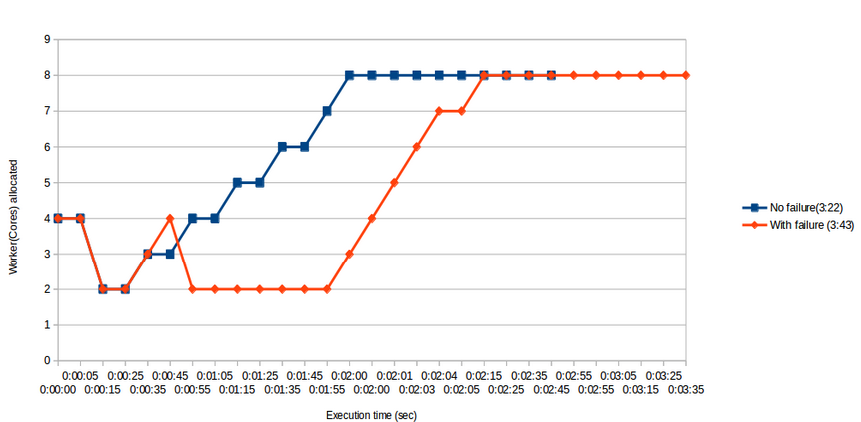
\includegraphics[width=\textwidth]{figures/adaptive.png}
  }
\end{frame}
\section{TODO}
\begin{frame}
  \frametitle{TODO}
  \begin{itemize}
    \item Co-work with CHT integrate with JPPF
  \end{itemize}

\end{frame}
\begin{frame}
  \frametitle{Integration with JPPF}
  \begin{itemize}[<+->]
      \only<1-2>{
      \item JPPF (Java Parallel Processing Framework) is a very popular open-source cluster management
        framework
        \begin{itemize}
          \item <.->Very easy to deploy
          \item <.->GUI monitoring tools
          \item <.->Active development
        \end{itemize}
      \item Doesn't support \emph{centralized} and
        \emph{node-aware} scheduling
      }
      \only<3->{
      \item Provides API for jobs set "filters" for a job -- to reject a
        node of from running that job
      \item Leveraging this API, we can somehow implement node-aware
        scheduling by \pause
        \begin{enumerate}
          \item Contact the system for scheduling information
          \item Get scheduled worker of the job
          \item Reject if this node is not scheduled
        \end{enumerate}
      }
  \end{itemize}
\end{frame}
\end{document}
